\documentclass[a4paper, 12pt,oneside]{article} 
%\documentclass[a4paper, 12pt,oneside,draft]{article} 
\usepackage{preamble}
%--------------------- ACTUAL FILE ---------------------- %
\begin{document} 
%%%
	\begin{titlepage}
    \newcommand{\HRule}{\rule{\linewidth}{0.5mm}} % Defines a new command for the horizontal lines, change thickness here
    
    \center  % Center everything on the page
     
    %----------------------------------------------------------------------------------------
    %   HEADING SECTIONS
    %----------------------------------------------------------------------------------------

    \vspace{3cm}
    \textsc{\LARGE École polytechnique fédérale de Lausanne}\\[1.5cm] % Name of your university/college
    
    \textsc{\Large Regression Methods Project Report}\\[0.5cm] % Major heading such as course name
    \textsc{\large Coin-Data Regression Study}\\[0.5cm] % Minor heading such as course title
    
    %----------------------------------------------------------------------------------------
    %   TITLE SECTION
    %----------------------------------------------------------------------------------------
    
    \HRule \\[0.4cm] % line above and under the title
    
    
    % Title of your document
    
    \HRule \\[1.5cm]
     
    %----------------------------------------------------------------------------------------
    %   AUTHOR SECTION
    %----------------------------------------------------------------------------------------
    
    \begin{minipage}{0.4\textwidth}
    \begin{flushleft} \large
    
    \emph{Authors:}\\
    Tara \textsc{Fjellman}\\
    Rayan \textsc{Harfouche}\\
    
    
    
    
    \end{flushleft}
    \end{minipage}
    ~
    \begin{minipage}{0.4\textwidth}
    \begin{flushright} \large
    
    \emph{Professor:} \\
    Anthony \textsc{Davison}\\
    \end{flushright}
    \end{minipage}\\[10cm]
    %
    
    
    %----------------------------------------------------------------------------------------
    %   LOGO SECTION
    %----------------------------------------------------------------------------------------
    
    
\includegraphics[width=0.4\linewidth]{Logo-1 .pdf}\\[1cm] 
    % Include a department/university logo - this will require the graphicx package
     
    %----------------------------------------------------------------------------------------
    
    \vfill % Fill the rest of the page with whitespace
    
    \end{titlepage} 
	% Add titlepage
	\clearpage
	\tableofcontents
	\thispagestyle{empty}
	% Add table of contents
	\clearpage
	\pagenumbering{arabic}
	\setcounter{page}{1}
	\section*{Abstract}
	\begin{itemize}
		\item context of the original paper (with their claims) 
		\item our addition/contribution/comment about it
	\end{itemize}
	\section{Introduction}
	\begin{itemize}
		\item unbalanced dataset 
		\item number of people and coins
		\item few people with many coins and few coins with many people
		\item inspection of same side rates show sign of possible person, coin and person-coin dependence
		\item mention the datasets that we used (with information in them)
		\item brief mention of types of models (GLM vs WLS and person-coin etc.). no formula, but description
	\end{itemize}
	\section{Analysis}
		\subsection{Model Comparison}
			In this section, we introduce and compare different models for the same side success rate. 

			Some GLMs with binomial responses and some WLS ones based on the ... approximation.
			
			Should explain no a priori response transformation ...
			
			For each, the considered formulas in terms of the covariates are:
			\begin{itemize}
				\item \texttt{1}, corresponding to a constant model.
				\item \texttt{1+C(person)}, corresponding to a model with the person as a covariate.
				\item \texttt{1+C(person)+C(coin)}, corresponding to a model with the person and the coin as covariates.
				\item \texttt{1+C(person)+C(coin)+C(person):C(coin)}, corresponding to a model with the person, the coin, and the interaction between the person and the coin as covariates.
			\end{itemize}
			* model 4 could seem redundant due to nesting-main effect, but we ....
			*  

			Should explain why eliminated some covariates ...
			\subsubsection{Tools For Selection}
			\begin{itemize}
				\item when to use AIC vs LRT ?
				\item citing a few things about LRT not miting overfitting 
				\item 
			\end{itemize}
			\subsubsection{WLS Approach}

			\subsubsection{GLM Approach}
			\lipsum[1]
			\begin{table}[htb]
				\centering
				\caption{Model comparison for different models.}
				\label{tab:model-comparison}
				\begin{tabular}{lccc}
				\toprule
				Model & Deviance & AIC & Model DF \\
				\midrule
				\texttt{1} & 3943.48 & 173.97 & 0 \\
				\texttt{1+C(person)} & 3677.51 & 0.00 & 46 \\
				\texttt{1+C(person)+C(coin)} & 3611.12 & 17.61 & 88 \\
				\bottomrule
				\end{tabular}
			\end{table}
			\lipsum[1]
			\begin{figure}[htb]
				\centering
				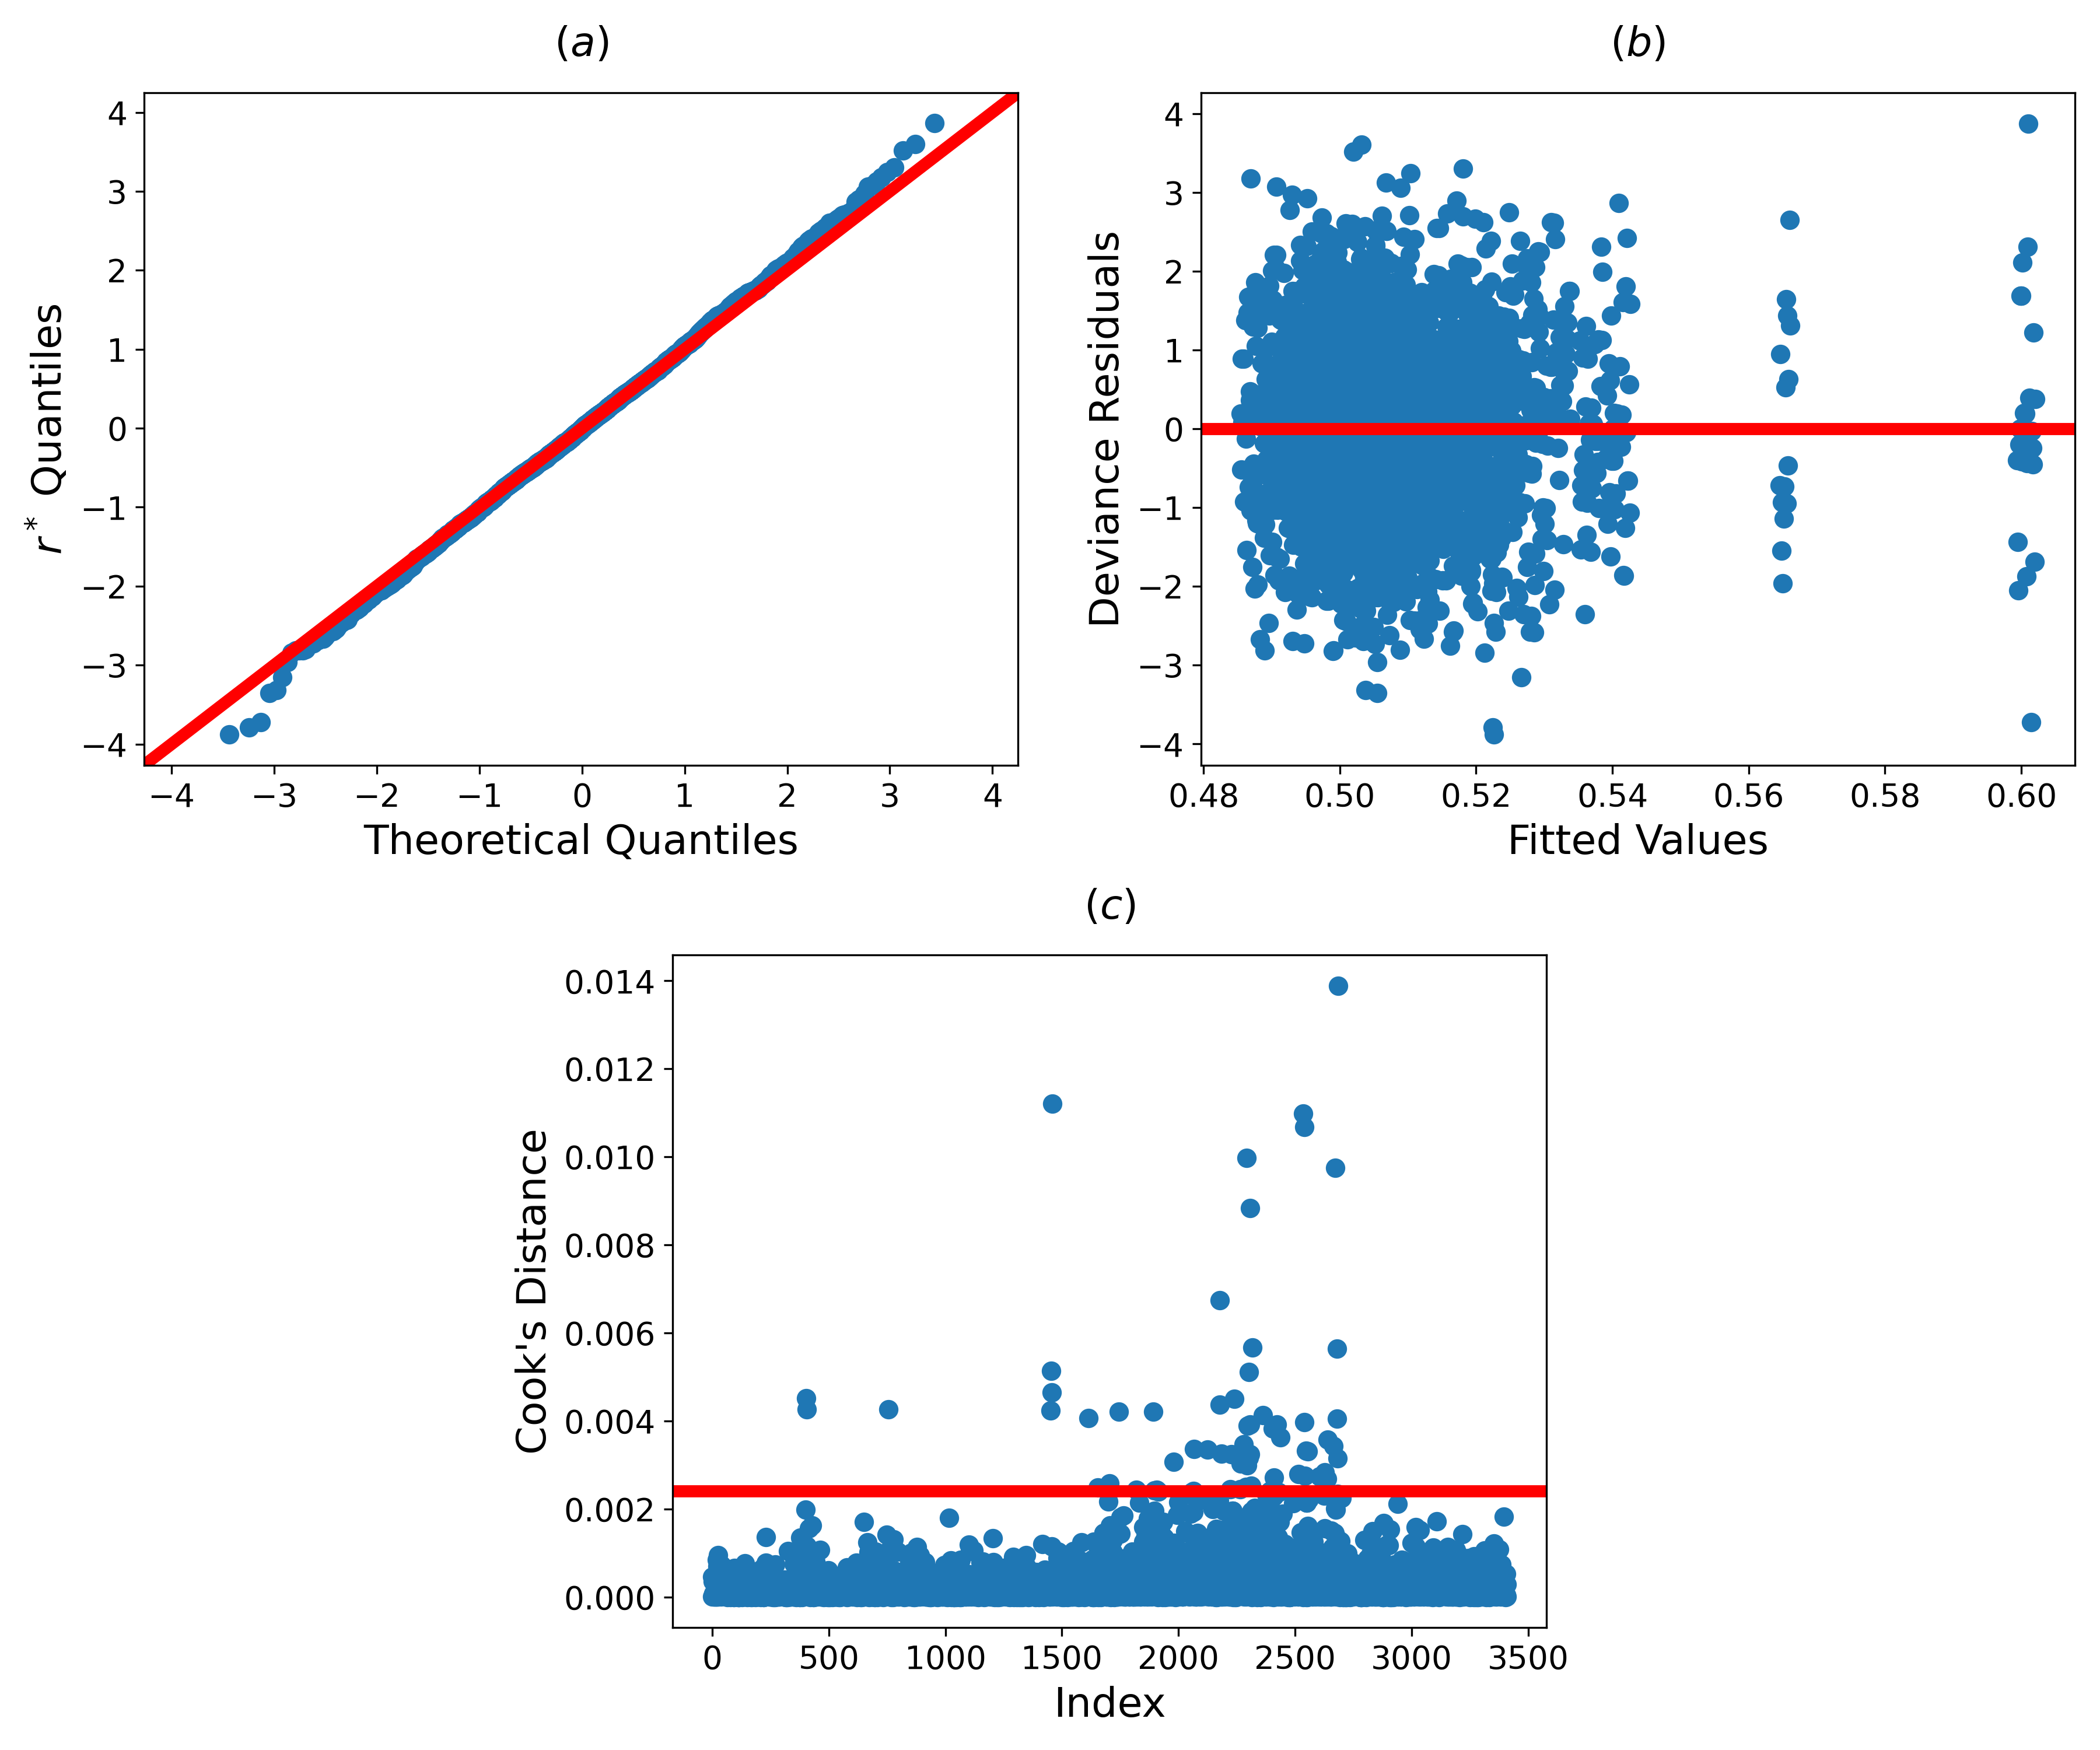
\includegraphics[width=0.85\textwidth]{GLM_diagnostics.png}
				\caption{Diagnostics for the selected GLM model. (a).}
				\label{fig:glm-diagnostic}
			\end{figure}
			\lipsum[1]
			\begin{table}[htb]
				\centering
				\caption{Likelihood ratio tests between models.}
				\label{tab:llr-comparison}
				\begin{tabular}{llc}
				\toprule
				Tested model & Restricted model & $p$-value \\
				\midrule
				\texttt{1+C(person)} & \texttt{1} & 0.00e+00 \\
				\texttt{1+C(person)+C(coin)} & \texttt{1+C(person)} & 9.61e-03 \\
				\bottomrule
				\end{tabular}
			\end{table}
		\subsection{Unusual Observations}
		\begin{figure}[htb]
			\centering
			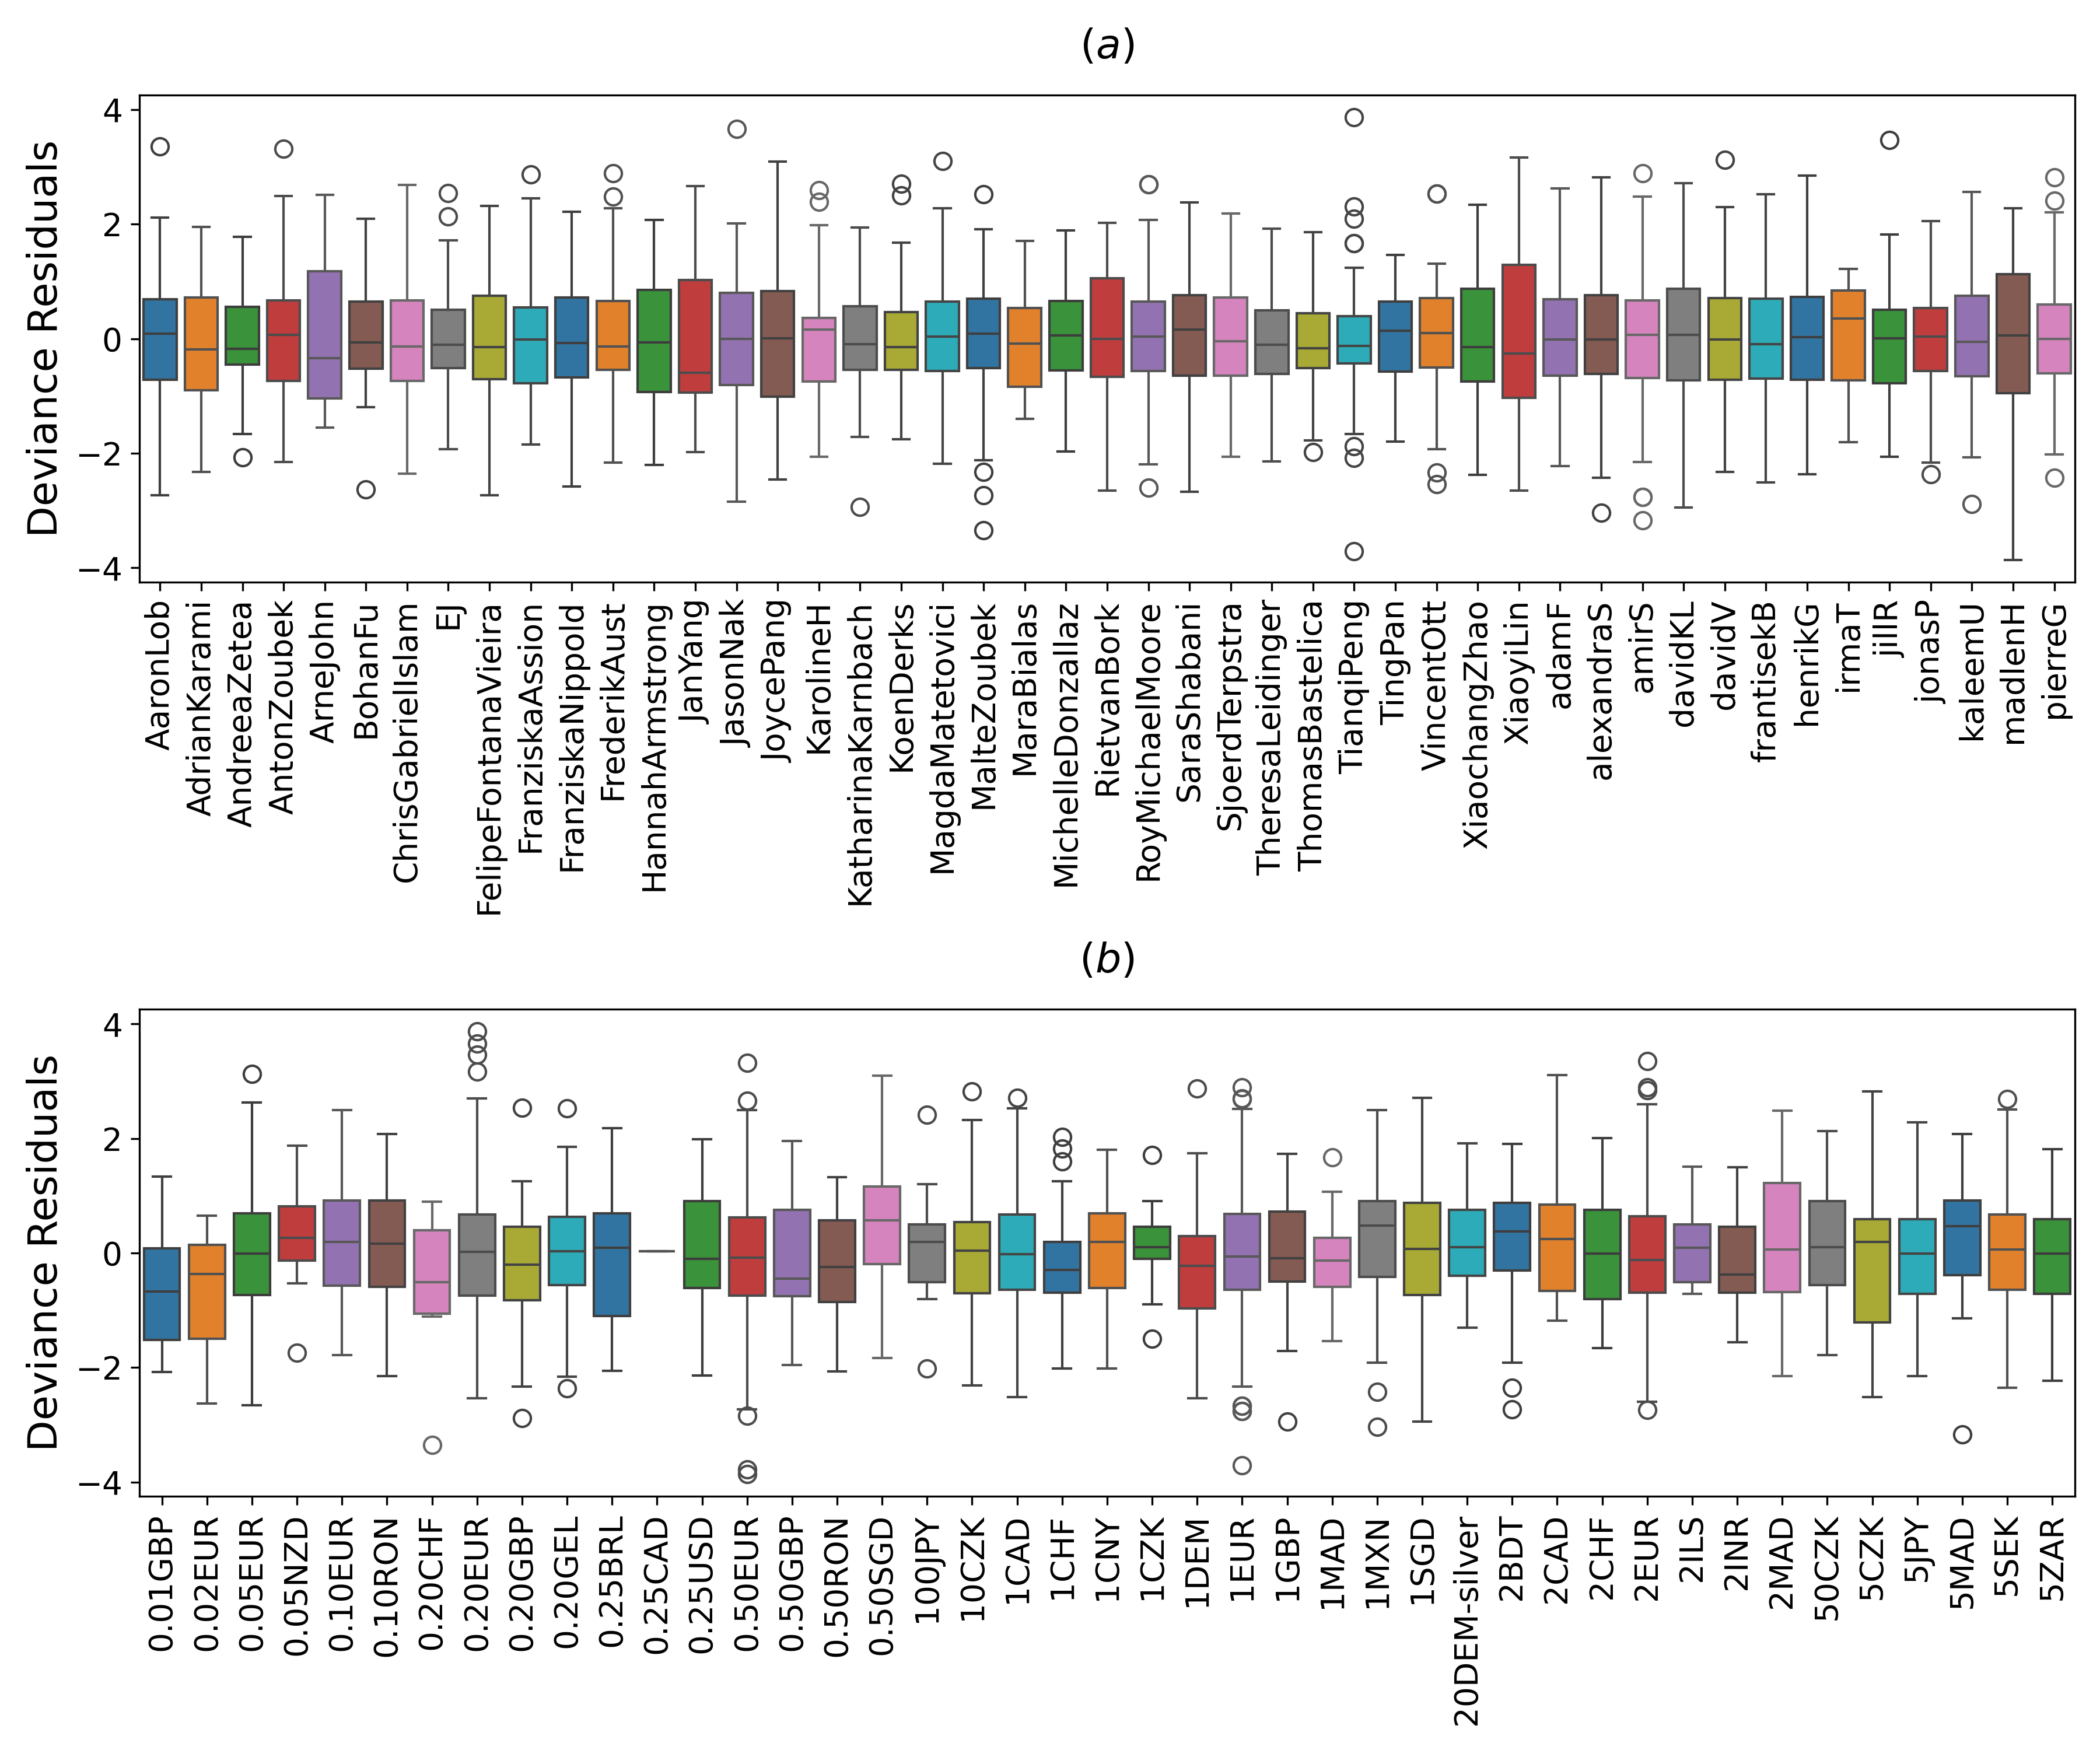
\includegraphics[width=0.85\textwidth]{dev_resid_vs_covariates.png}
			\caption{Dev-resid as a function of (a) person and (b) coin.}
			\label{fig:dev-resid-vs-covariates}
		\end{figure}

		\subsection{Zoom on Learning Effects}
		\begin{itemize}
			\item bias comes from start
			\item amount of bias (considerable)
			\item wobble interpretation (consistent with physical model, citing the paper)
		\end{itemize}
		\lipsum[1]
		\begin{figure}[htb]
			\centering
			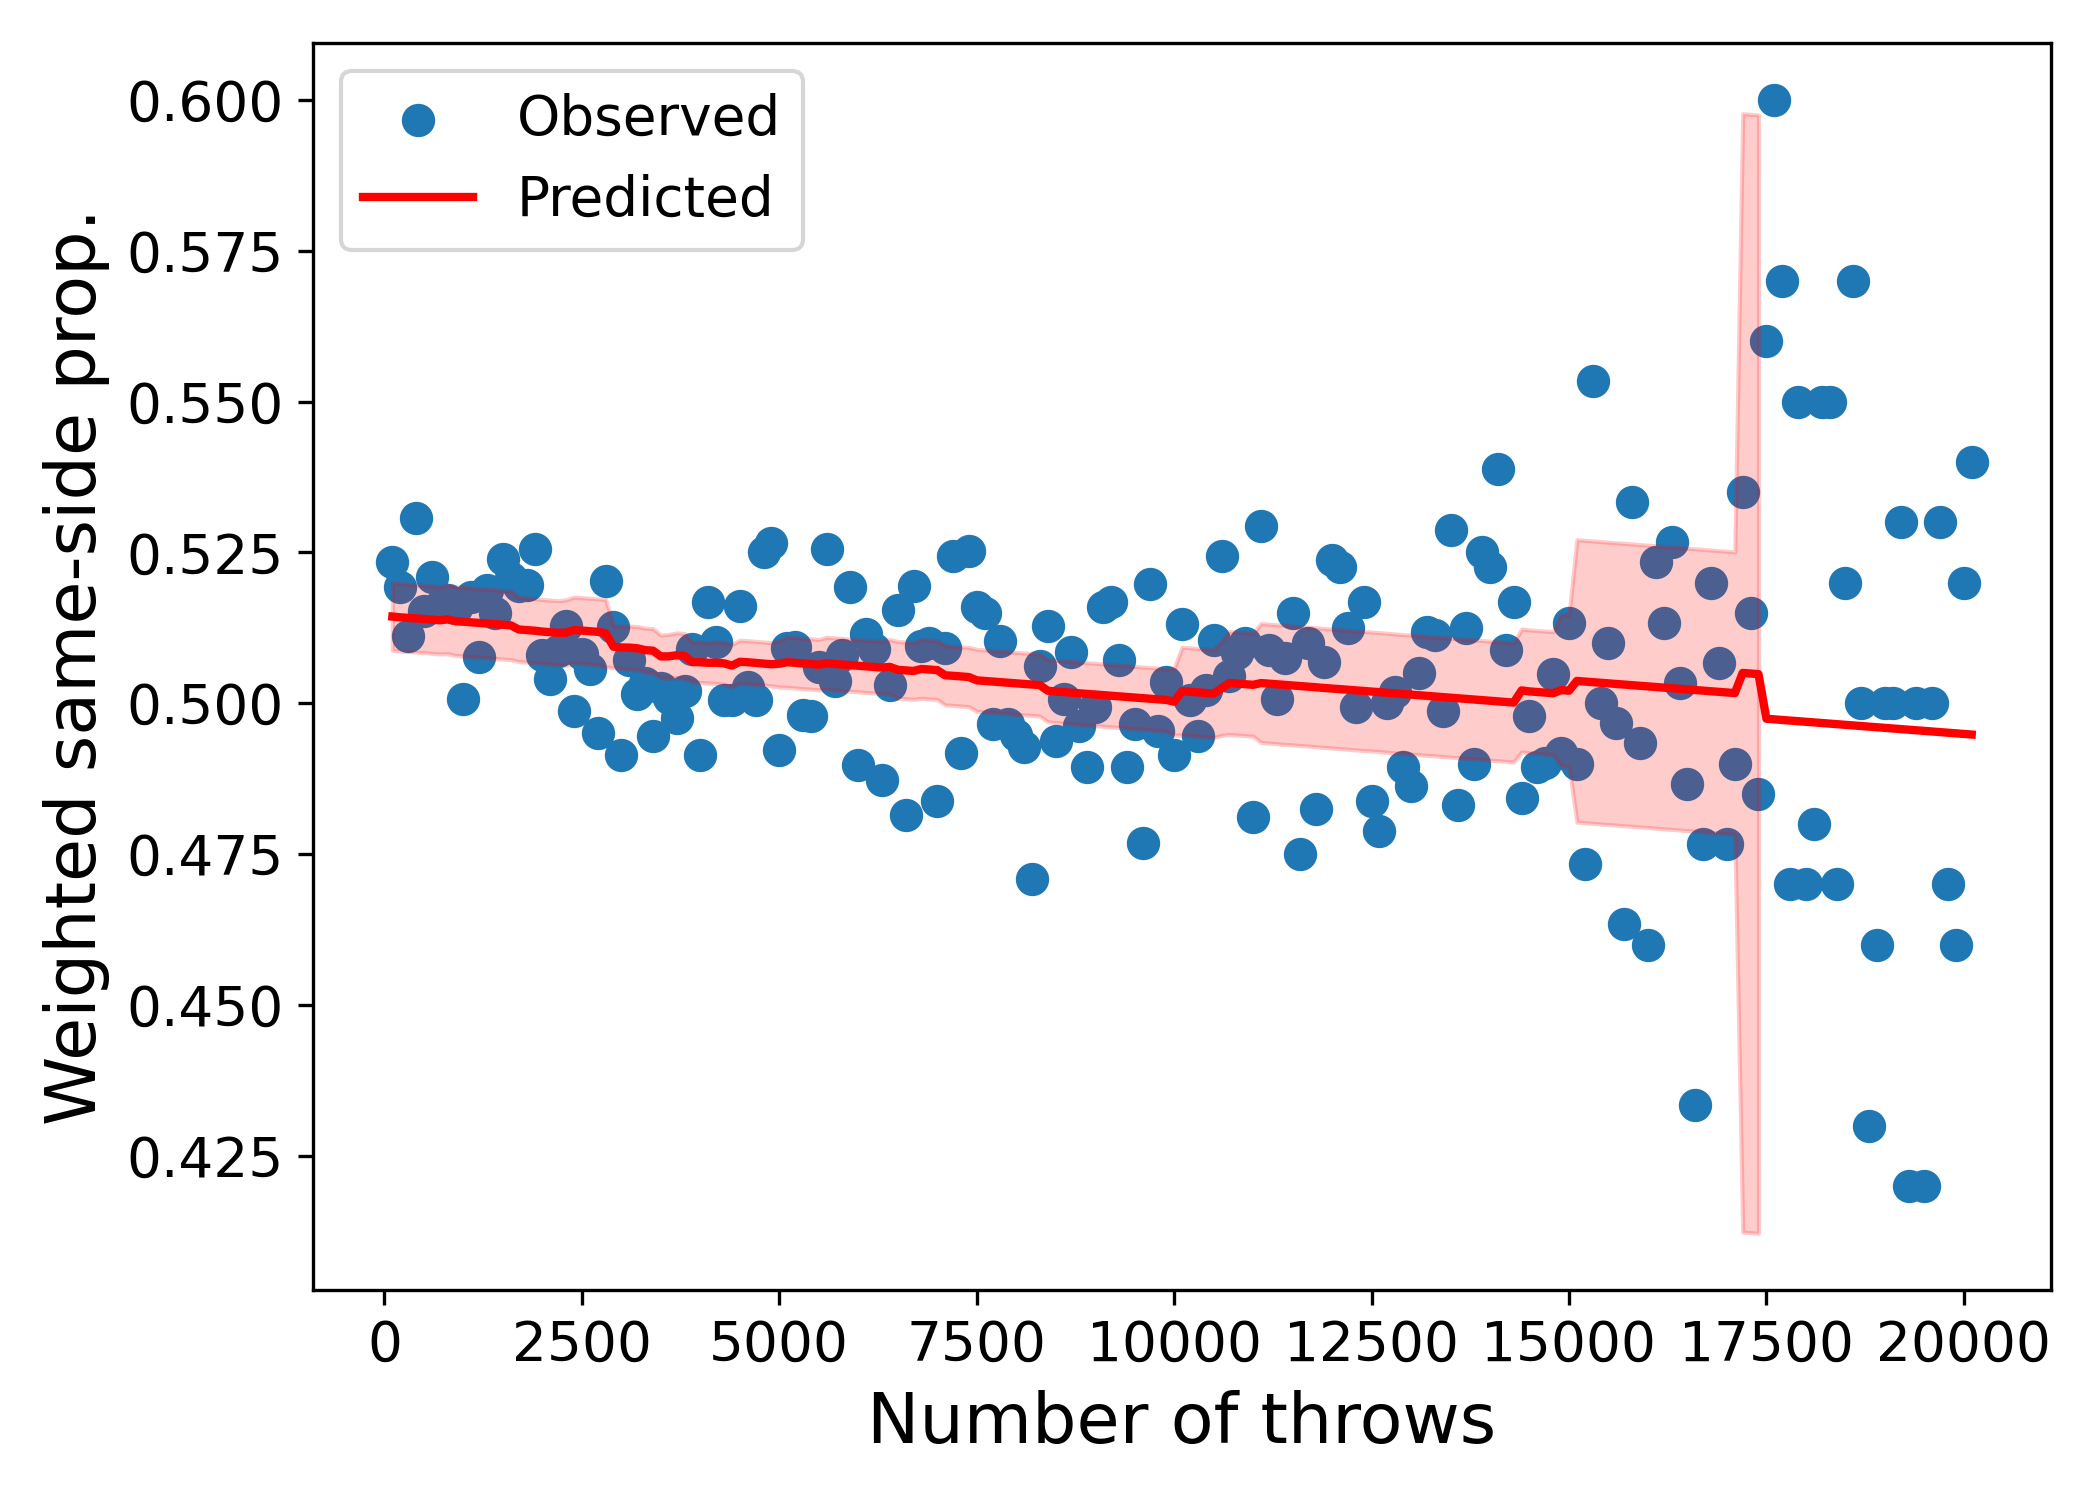
\includegraphics[width=0.5\textwidth]{learning_effects.png}
			\caption{Learning effects.}
			\label{fig:learning-effects}
		\end{figure}
		\subsection{Memory Effects ??}

	\section{Discussion}
	\section{Conclusion}
	\section*{Acknowledgements}
>>>>>>> 89d664ea2c5b851e9bd4b8dc11130acbb147cce6
	\section*{References}
	%\appendix
	%	\section{Runtime Estimation}\label{appendix:runtime_estimation}
%%%
\end{document} 